\documentclass[12pt,compress]{beamer}
\usepackage[utf8x]{inputenc}
\usepackage[ngerman]{babel}
\usepackage{color}
\usepackage{hyperref}
\usepackage{scrextend}
\usepackage{kmath,kerkis}
\usepackage{listings}

\usetheme{Boadilla}
\setbeamertemplate{footline}

\usecolortheme{lily}
\usefonttheme{serif}
\useinnertheme{circles}
\setbeamercovered{transparent}
\beamertemplatenavigationsymbolsempty

\definecolor{darkgreen}{rgb}{0,0.5,0}
\definecolor{darkblue}{RGB}{20,20,155}
\definecolor{purple}{RGB}{51,51,178}

\hypersetup{
    bookmarks=true,
    unicode=true,
    pdftoolbar=true,
    pdfmenubar=true,
    pdffitwindow=false,
    pdfstartview={FitH},
    pdftitle={Dark Corners of C},
    pdfauthor={Michael Hartmann},
    pdfcreator={vim},
    pdfproducer={pdflatex},
    pdfkeywords={C} {undefined behavior} {LIT} {Linux} {Infotag} {Augsburg} {LUGA},
    pdfnewwindow=true,
    colorlinks=true,
    linkcolor=black,
    citecolor=green,
    filecolor=magenta,
    urlcolor=darkgreen
}

\lstset{ %
  commentstyle=\color{darkblue}, % comment style
  keepspaces=true,               % keeps spaces in text, useful for keeping indentation of code (possibly needs columns=flexible)
  keywordstyle=\color{red},      % keyword style
  basicstyle=\ttfamily\small,
  language=C,                    % the language of the code
  numbers=left,                  % where to put the line-numbers; possible values are (none, left, right)
  numbersep=5pt,                 % how far the line-numbers are from the code
  numberstyle=\tiny,             % the style that is used for the line-numbers
}


\title{Dark Corners of C}
\institute{16. Augsburger Linux-Infotag}
\author{Michael Hartmann}
\date{22. April 2017}


\titlegraphic{
\includegraphics[scale=0.2]{images/logo.png}}

\begin{document}

\begin{frame}
    \titlepage
\end{frame}

\section*{Einleitung}
\frame {
    \frametitle{Mein Weg zu C}
    
    \begin{center}
    \only<1>
    {
    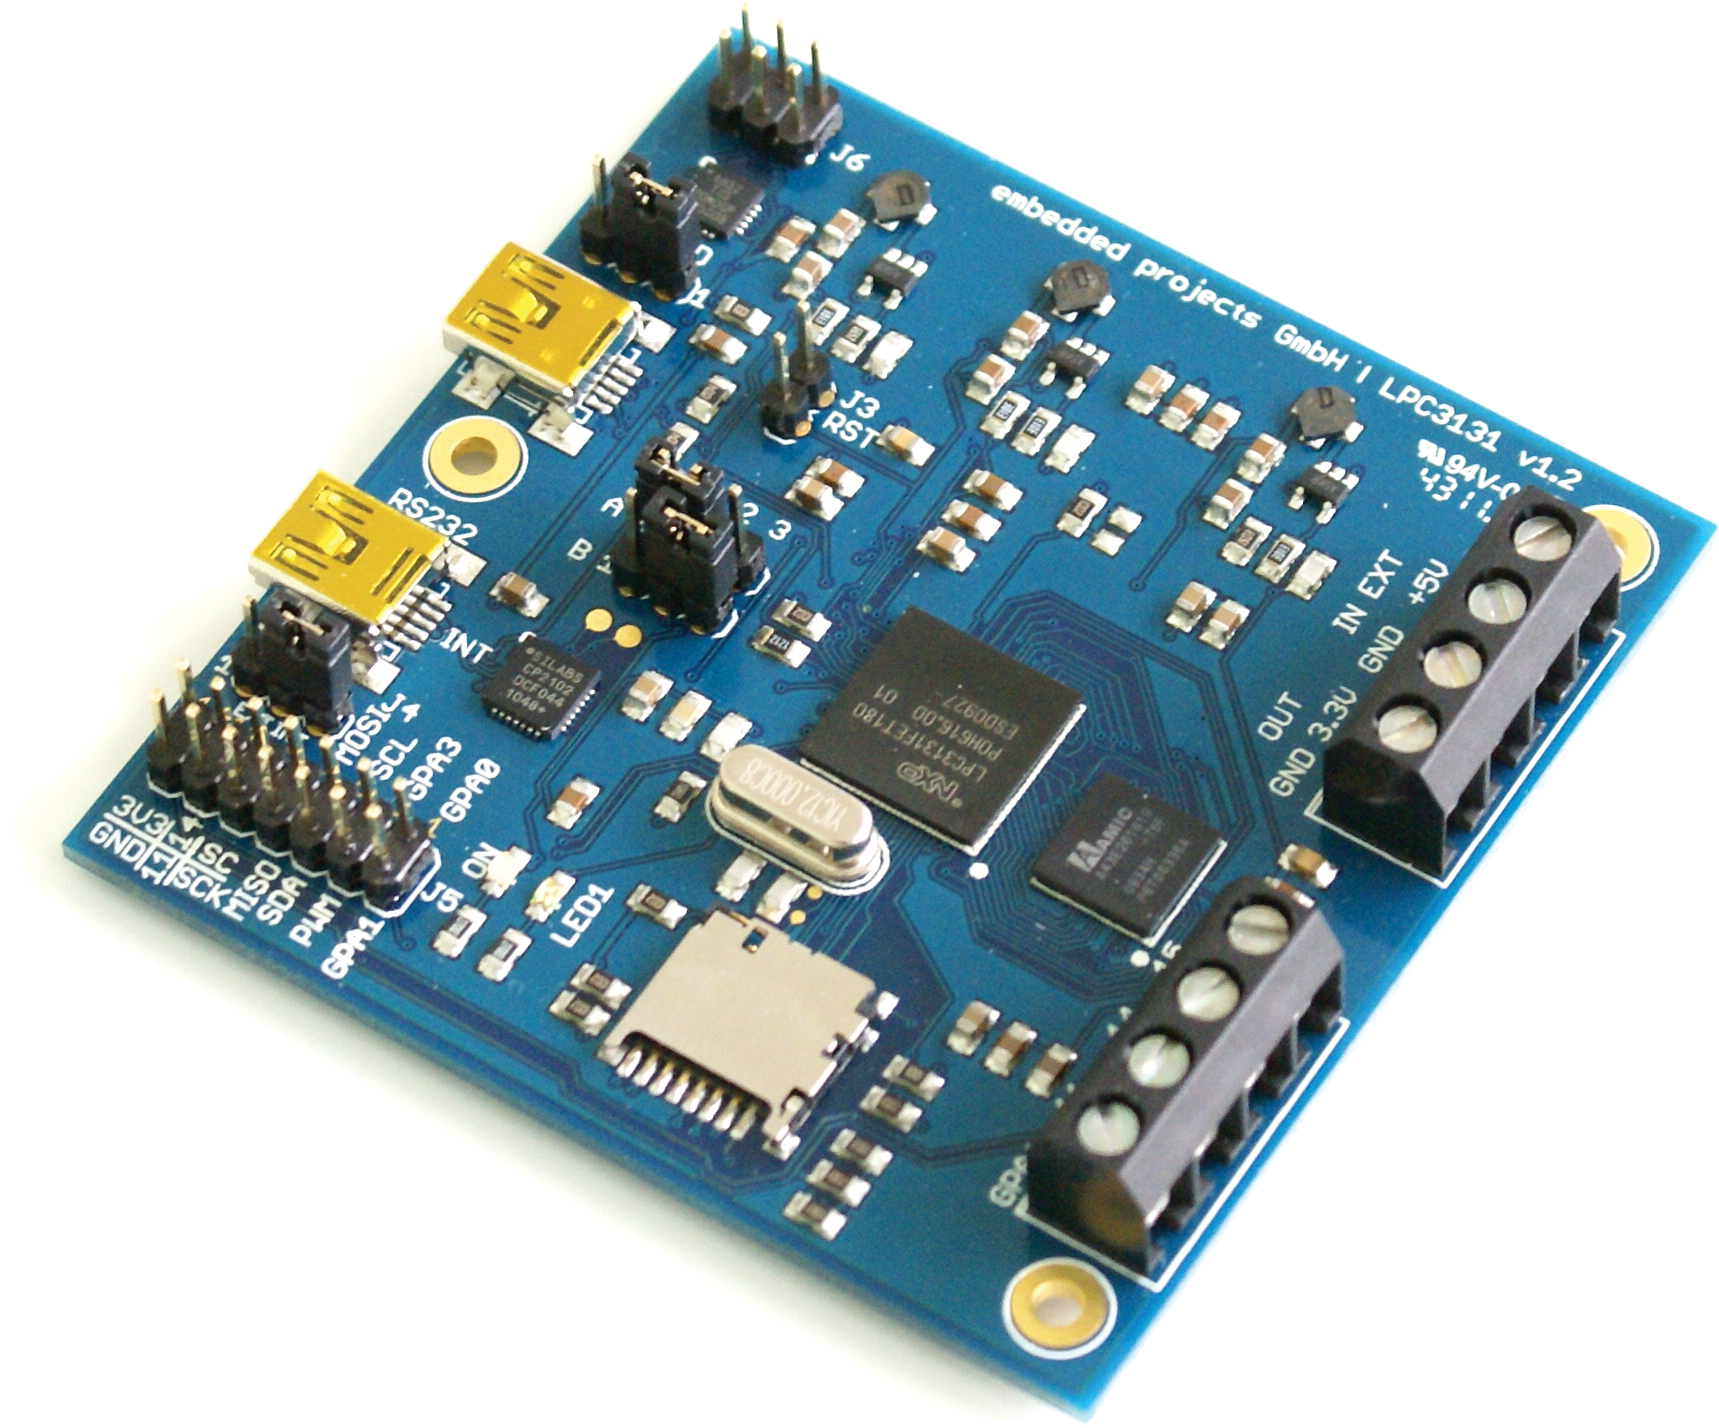
\includegraphics[scale=0.4]{images/gnublin.png}
    }

    \only<2>
    {
    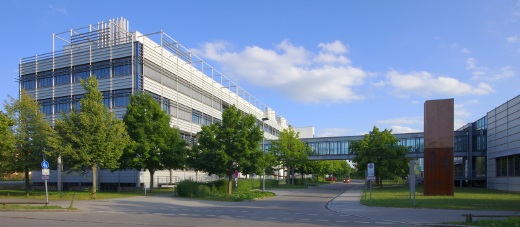
\includegraphics[scale=0.6]{images/physik.jpg}
    }
    \end{center}
}

\frame {
    \frametitle{TIOBE Programming Community Index}

    \begin{center}
    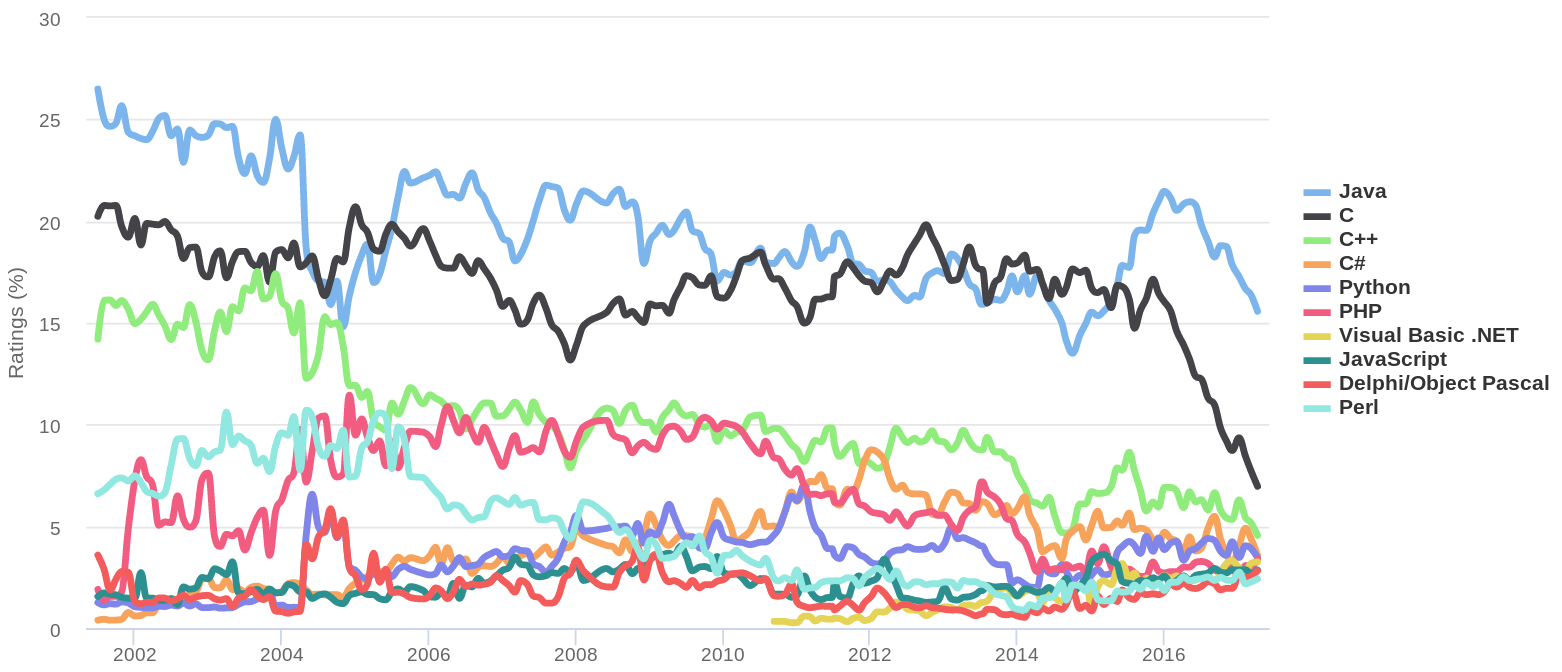
\includegraphics[scale=0.3]{images/tiobe.png}
    \end{center}
}

\section{Die Sprache}

\frame {
    \begin{center}
    \color{purple}
    \Huge Die Sprache
    \end{center}
}

\subsection{Keywords}
\frame {
    \frametitle{Keywords}

\texttt{{\only<2->{\color{red}}auto}
    break
    case
    char
    const
    continue
    default
    do
    double
    else
    enum
    extern
    float
    for
    goto
    if
    int
    long
    register
    return
    short
    {\only<3>{\color{red}}signed}
    sizeof
    static
    struct
    switch
    typedef
    union
    unsigned
    void
    volatile
    while 
    }
}


\begin{frame}[fragile]
\frametitle{Kommentare}

\begin{lstlisting}
int x = 2, y = 10, z;
int *p = &x; 

/* Fehler */
z = y/*p;

/* y/(*p) */
z = y/ *p;
\end{lstlisting}
\end{frame}

\begin{frame}[fragile]
\frametitle{Kommentare}

\begin{lstlisting}
int x = 10, y;
y = x//* kommentar */2;
printf("%d\n", y);
\end{lstlisting}

\vfill

\begin{center}
C89: 5 \quad\quad C99: Fehler
\end{center}

\end{frame}

\begin{frame}
    \frametitle{VLA}

    Variable length arrays
    \begin{itemize}
    \item mandatory in C99
    \item optional in C11 (?!)
    \end{itemize}

    \vfill

    \only<2,3>
    {{\it For such an object that does have a variable length array type, its
    lifetime extends from the declaration of the object until execution of the
    program leaves the scope of the declaration. If the scope is entered
    recursively, a new instance of the object is created each time. The initial
    value of the object is indeterminate.}} 

    \vfill

    \only<3>
    {
        \begin{center}
    {\Large    Stack? \quad Heap?    }
        \end{center}
    }

\end{frame}

\subsection{Variable length arrays}
\begin{frame}[fragile]
    \frametitle{VLA}

\begin{lstlisting}
double sum(size_t nmax) {
    double sum = 0, buf[nmax];

    for(size_t i = 0; i < nmax; i++)
        buf[i] = 1./(1+i);

    for(size_t i = 0; i < nmax; i++)
        sum += buf[i];

    return sum;
}

sum(1000);     // 5.18738...
sum(10000000); // Segmentation Fault
\end{lstlisting}
\end{frame}


\section{Macros}

\frame {
    \begin{center}
    \color{purple}
    \Huge Macros
    \end{center}
}

\begin{frame}[fragile]
\frametitle{Macros}

\begin{lstlisting}
#define SQUARE(x) x*x

SQUARE(2+1);
\end{lstlisting}

\end{frame}

\begin{frame}[fragile]
\frametitle{Macros}

\begin{lstlisting}
#define SQUARE(x) x*x

SQUARE(2+1); // 2+1*2+1 = 5
\end{lstlisting}
\end{frame}


\begin{frame}[fragile]
\frametitle{Macros}

\begin{lstlisting}
#define SQUARE(x) (x)*(x)

SQUARE(2+1);
\end{lstlisting}
\end{frame}


\begin{frame}[fragile]
\frametitle{Macros}

\begin{lstlisting}
#define SQUARE(x) (x)*(x)

SQUARE(2+1); // (2+1)*(2+1) = 9
\end{lstlisting}
\end{frame}


\begin{frame}[fragile]
\frametitle{Macros}

\begin{lstlisting}
#define SQUARE(x) (x)*(x)

SQUARE(3000000000); // -494665728
\end{lstlisting}
\end{frame}

\begin{frame}[fragile]
\frametitle{Macros}

\begin{lstlisting}
#define SQUARE(x) (x)*(x)

SQUARE(3000000000); // -494665728
SQUARE(3000000000.); // 9e18
\end{lstlisting}
\end{frame}

\begin{frame}[fragile]
\frametitle{Macros}

\begin{lstlisting}
#define MIN(X, Y)  ((X) < (Y) ? (X) : (Y))

min(a,b++);
min(x+y,foo(z));
\end{lstlisting}
\end{frame}

\begin{frame}[fragile]
\frametitle{Macros}

\begin{lstlisting}
#define MIN(X, Y)  ((X) < (Y) ? (X) : (Y))

min(a,min(b,min(c,d)));

/* becomes */
((a) < (((b) < (((c) < (d) ? (c) : (d))) ?
(b) : (((c) < (d) ? (c) : (d))))) ?
(a) : (((b) < (((c) < (d) ?
(c) : (d))) ? (b) : (((c) < (d) ?
(c) : (d))))));
\end{lstlisting}
\end{frame}

\begin{frame}[fragile]
\frametitle{Macros}

\begin{lstlisting}
#define assert(e) \
	if(!e) panic(__FILE__, __LINE__)

int x = 0, y = 1;
assert(x > y);

/* becomes */
if(!0 > 1) /* 1 > 1 */
    panic(...);
\end{lstlisting}
\end{frame}


\begin{frame}[fragile]
\frametitle{Macros}

\begin{lstlisting}
#define assert(e) \
	if(!(e)) panic(__FILE__, __LINE__)

if(x > 0 && y > 0)
    assert(x > y);
else
    assert(y > x);

/* becomes */
if(x > 0 && y > 0)
    if(!(x > y))
        panic(...);
    else
        if(!(y > x))
            panic(...);
\end{lstlisting}
\end{frame}


\begin{frame}[fragile]
\frametitle{Macros}

\begin{lstlisting}
#define assert(e) \
	{ if(!(e)) panic(__FILE__, __LINE__); }

if(x > 0 && y > 0)
    assert(x > y);
else
    assert(y > x);

/* becomes */
if(x > 0 && y > 0)
    { if(!(x > y)) panic(...); };
else
    { if(!(y > x)) panic(...); };
\end{lstlisting}
\end{frame}


\begin{frame}[fragile]
\frametitle{Macros}

\begin{lstlisting}
/* correct */
#define assert(e) \
  (void)((e)||panic(__FILE__, __LINE__))

/* should also work */
#define assert(e) \
	do { if(!(e)) panic(__FILE__, __LINE__); } \
		while(0)
\end{lstlisting}
\end{frame}

\section{Standardbibliothek}

\frame {
    \begin{center}
    \color{purple}
    \Huge Standardbibliothek
    \end{center}
}

\begin{frame}[fragile]
\frametitle{\texttt{gets}}

\begin{lstlisting}
char *gets(char *s);
\end{lstlisting}

\vfill

Never use \texttt{gets()}.  Because it is impossible to tell without knowing
the data in advance how many characters \texttt{gets()} will read, and because
\texttt{gets()} will continue to store characters past the end of the buffer,
it is extremely dangerous to use.  It has been used to break computer security.
\end{frame}

\begin{frame}[fragile]
\frametitle{\texttt{realloc}}

\begin{lstlisting}
char *buf = (char *)malloc(elems*sizeof(char));
if(buf == NULL)
	...

...

buf = realloc(buffer, newelems*sizeof(char));
if(buf == NULL)
    /* Memory leak */
    ...
\end{lstlisting}
\end{frame}


\frame {
\frametitle{\texttt{lgamma}}

\only<1>
{
The \texttt{lgamma()} function returns the natural logarithm of the absolute
value of the Gamma function.  The sign of the Gamma function is returned in the
external integer \texttt{signgam} declared in \texttt{<math.h>}. [$\dots$]
}
\only<2->
{
Since using a constant location \texttt{signgam} is not thread-safe, the functions
\texttt{lgamma\_r()}, \texttt{lgammaf\_r()}, and \texttt{lgammal\_r()} have been
introduced; they return the sign via the argument \texttt{signp}.
}

\only<3>
{
\vfill
\texttt{lgamma\_r(), lgammaf\_r(), lgammal\_r()}: \\
\quad\quad\quad           \texttt{\_BSD\_SOURCE || \_SVID\_SOURCE}
}
}


\begin{frame}[fragile]
\frametitle{\texttt{errno}}

\begin{lstlisting}
library_function();
if(errno)
    /* Fehlerbehandlung */
\end{lstlisting}
\end{frame}

\begin{frame}[fragile]
\frametitle{\texttt{errno}}

\begin{lstlisting}
errno = 0;
library_function();
if(errno)
    /* Fehlerbehandlung */
\end{lstlisting}
\end{frame}

\begin{frame}[fragile]
\frametitle{\texttt{errno}}

\begin{lstlisting}
ret = library_function();
if(error_condition)
    /* inspect errno */
\end{lstlisting}
\end{frame}

\section{Undefined behavior}

\frame {
    \begin{center}
    \color{purple}
    \Huge Undefined behavior
    \end{center}
}

\begin{frame}[fragile]
\frametitle{Undefined behavior}

\begin{lstlisting}
int buffer[] = { 1,2,3 };
int x = buffer[3];
printf("%d\n", x);
\end{lstlisting}

\vfill

mögliche Ausgabe
\begin{itemize}
\item 0
\item 42
\item -1
\item \texttt{Poste Browserverlauf auf Facebook...}
\end{itemize}
\end{frame}

\frame {
\frametitle{Was ist undefiniert?}

Z.B.:
\begin{itemize}
\item lesen uninitialisierter Variablen
\item Dereferenzieren von wilden Pointern, Out of Bounds Array Accesses
\item Dereferenzieren des \texttt{NULL} Pointers
\item Casting: \texttt{int *} nach \texttt{float *} casten und Pointer dereferenzieren
\item Integer Division durch 0
\item {\it An unmatched ‘ or ” character is encountered on a logical source line during tokenization.}
\item ...
\end{itemize}
}

\begin{frame}[fragile]
\frametitle{Kürzeste Funktion mit undefinierten Verhalten}

\begin{lstlisting}
int f(int x) { return -x; }

int main(void)
{
    printf("f(%d)=%d\n", INT_MIN, f(INT_MIN));
    return 0;
}
\end{lstlisting}

\vfill

auf meinem Rechner:

\texttt{f(-2147483648)=-2147483648}

\end{frame}

\begin{frame}[fragile]
\frametitle{Vorteile}

\begin{itemize}
\item uninitialisierte Variablen: \texttt{memset} für Arrays teuer...
\item Signed integer overflows:
\begin{lstlisting}
int i;
i+1 > i; /* true */ 
i*2/2; /* i */

/* Schleife wird N+1 mal ausgefuehrt */
for(i = 0; i <= N; ++i) {
	...
}
\end{lstlisting}
\item Out of Bounds Array Access: Checks zur Laufzeit teuer, würde Binärkompatibilität mit alten Programmen brechen
\end{itemize}
\end{frame}


\begin{frame}[fragile]
\frametitle{Undefiniertes Verhalten und Optimierungen}

\begin{lstlisting}
void f(int *P) {
    int dead = *P;
    if (P == NULL)
        return;
    *P = 4;
}
\end{lstlisting}

\vfill
Zwei Optimierungen:
\begin{itemize}
\item Dead Code Elimination
\item Redundant Null Check Elimination:
\end{itemize}

\vfill

Verhalten hängt von der Reihenfolge der Optimierungen ab!
\end{frame}


\begin{frame}[fragile]
\frametitle{Undefiniertes Verhalten und Optimierungen}

Dead Code Elimination:

\vfill

\begin{lstlisting}
void f(int *P) {
    int dead = *P; /* dead code */
    if (P == NULL)
        return;
    *P = 4;
}
\end{lstlisting}
\end{frame}


\begin{frame}[fragile]
\frametitle{Undefiniertes Verhalten und Optimierungen}

Redundant Null Check Elimination:

\vfill

\begin{lstlisting}
void f(int *P) {
    if (P == NULL) /* Check nicht redundant */
        return;
    *P = 4;
}
\end{lstlisting}
\end{frame}


\begin{frame}[fragile]
\frametitle{Undefiniertes Verhalten und Optimierungen}

Code mit zuerst DCE und danach RNCE:

\vfill

\begin{lstlisting}
void f(int *P) {
    if (P == NULL)
        return;
    *P = 4;
}
\end{lstlisting}
\end{frame}


\begin{frame}[fragile]
\frametitle{Undefiniertes Verhalten und Optimierungen}

\begin{center}
Und jetzt anders herum!
\end{center}

\end{frame}


\begin{frame}[fragile]
\frametitle{Undefiniertes Verhalten und Optimierungen}

Redundant Null Check Elimination:

\vfill

\begin{lstlisting}
void f(int *P) {
    int dead = *P;
    if (P == NULL) /* P darf nicht NULL sein */
        return;
    *P = 4;
}
\end{lstlisting}
\end{frame}


\begin{frame}[fragile]
\frametitle{Undefiniertes Verhalten und Optimierungen}

Dead code elimination:

\vfill

\begin{lstlisting}
void f(int *P) {
    int dead = *P; /* dead code */
    *P = 4;
}
\end{lstlisting}
\end{frame}


\begin{frame}[fragile]
\frametitle{Undefiniertes Verhalten und Optimierungen}

Code mit zuerst RNCE und danach DCE:

\vfill

\begin{lstlisting}
void f(int *P) {
    *P = 4;
}
\end{lstlisting}
\end{frame}


\begin{frame}[fragile]
\frametitle{Undefiniertes Verhalten und Security}
\begin{lstlisting}
void process_something(int size) {
    /* check for integer overflow */
    if (size > size+1)
        abort();
    
    ...

    /* alles ok hier */
    char *string = malloc(size+1);
    read(fd, string, size);
    string[size] = 0;
    do_something(string);
    free(string);
}
\end{lstlisting}
\end{frame}


\begin{frame}[fragile]
\frametitle{Undefiniertes Verhalten und Security}

Signed integer Overflows sind undefiniert...

\vfill

Nach Optimieren sieht der Code vermutlich so aus:

\vfill

\begin{lstlisting}
void process_something(int size) {
    ...

    /* alles ok hier */
    char *string = malloc(size+1);
    read(fd, string, size);
    string[size] = 0;
    do_something(string);
    free(string);
}
\end{lstlisting}
\end{frame}

\begin{frame}[fragile]
\frametitle{Real-world Beispiel}

\begin{lstlisting}
void __devexit agnx_pci_remove (struct pci_dev *pdev)
{
    struct ieee80211_hw *dev = pci_get_drvdata(pdev);
    struct agnx_priv *priv = dev->priv; 

    if (!dev)
        return;

    ...
}
\end{lstlisting}
\end{frame}

\frame {
    \frametitle{gcc}


\texttt{-fdelete-null-pointer-checks}: \\
\begin{addmargin}[1em]{2em}
Assume that programs cannot safely dereference null pointers, and that no code or data element resides there.  This enables simple constant folding optimizations at all optimization levels.  In
addition, other optimization passes in GCC use this flag to control global dataflow analyses that eliminate useless checks for null pointers; these assume that if a pointer is checked after it
has already been dereferenced, it cannot be null.

\vfill

Note however that in some environments this assumption is not true.  Use
\texttt{-fno-delete-null-pointer-checks} to disable this optimization for programs that
depend on that behavior.
\end{addmargin}

}


\begin{frame}[fragile]
\frametitle{Undefiniertes Verhalten und Debugging...}

\begin{lstlisting}
void f(bool b) {
    if(b)
        printf("true\n");
    else
        printf("false\n");
}

int main(int argc, char *argv[]) {
    bool *p = (bool *)malloc(sizeof(bool));

    f(*p);
    f(!*p);

    return 0;
}
\end{lstlisting}
\end{frame}

\frame {
\frametitle{Undefiniertes Verhalten und Debugging...}

\texttt{\$ gcc -Wall -Wextra -O2 truefalse.c  \\
\$ ./a.out  \\
false \\
true \\
\$ clang -Wall -Wextra -Oz truefalse.c  \\
\$ ./a.out  \\
false \\
false
}
}

\section{Workarounds}

\frame {
    \begin{center}
    \color{purple}
    \Huge Workarounds
    \end{center}
}

\frame {
    \frametitle{Workarounds}

    \begin{itemize}
    \item Compiler Warnungen: \texttt{-Wall -Wextra}
    \item Clang Static Analyzer
    \item Clang's \texttt{-fsanitize} Option
    \item valgrind
    \item gcc integer overflow builtins:
    
    \texttt{\_\_builtin\_add\_overflow},
    \texttt{\_\_builtin\_mul\_overflow}, ...
    \end{itemize}
}

\frame {
    \frametitle{Clang Static Analyzer}

    \begin{center}
    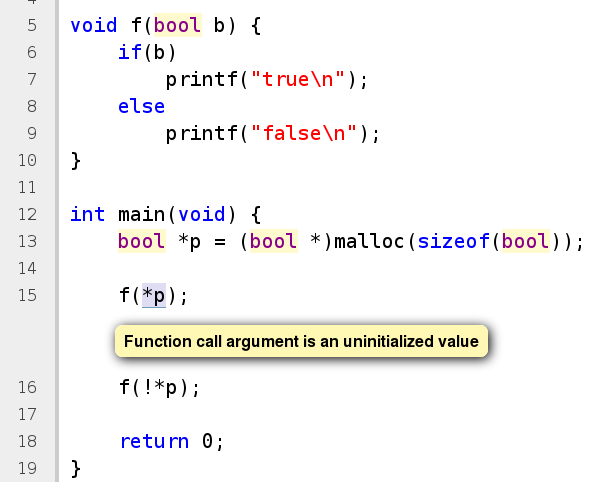
\includegraphics[scale=0.5]{images/clang-static.png}
    \end{center}
}

\frame {
    \frametitle{valgrind}

{ \small
\texttt{\$ valgrind ./a.out \\
\ \\
==27502== Conditional jump or move depends on uninitialised value(s) \\
==27502==    at 0x400573: f (in a.out) \\
==27502==    by 0x400467: main (in a.out) \\
==27502==  \\
false \\
...
}
}
}

\frame {
    \frametitle{Clang's \texttt{-fsanitize} Option}

{ \small
\texttt{\$ clang -fsanitize=undefined,memory truefalse.c \\
\$ ./a.out  \\
==27607== WARNING: MemorySanitizer: use-of-uninitialized-value \\
\quad\quad\#0 0x7f53cadbd873 (a.out+0x94873) \\
\quad\quad\#1 0x7f53c9c3cb44 (libc.so.6+0x21b44) \\
\quad\quad\#2 0x7f53cadbd38c (a.out+0x9438c) \\
\  \\
SUMMARY: MemorySanitizer: use-of-uninitialized-value ??:0 ?? \\
Exiting
}
}
}

\frame {
    \begin{center}
    \color{purple}
    \Huge Vielen Dank für die Aufmerksamkeit!
    \end{center}

    \vfill

    {
    Credits and links:
    \begin{itemize}
    \item \hyperlink{http://blog.llvm.org/2011/05/what-every-c-programmer-should-know.html}{What Every C Programmer Should Know About Undefined (LLVM)}
    \item \hyperlink{http://blog.regehr.org/archives/213}{A Guide to Undefined Behavior in C and C++ (Embedded in Academia)}
    \item \hyperlink{https://markshroyer.com/2012/06/c-both-true-and-false/}{Both true and false (mark shroyer, dot com)}
    \item \hyperlink{http://tinyurl.com/mrv44kk}{Some dark corners of C (Rob Kendrick)}
    \item \hyperlink{https://clang-analyzer.llvm.org/}{Clang Static Analyzer}
    \end{itemize}
    }
}

\end{document}
\grid
